\section{Casi d'uso} 
\subsection{Attori dei casi d'uso}
\subsubsection{Attori primari}
\begin{figure}[h]
	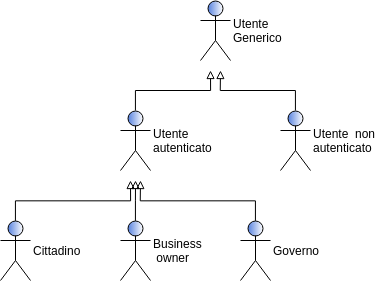
\includegraphics[width=7cm]{res/images/attori_primari.png}
	\centering
	\caption{Gerarchia attori primari}
\end{figure}
\begin{description}[style=nextline]
	\item[Utente Generico]
	Si riferisce ad un utente generico che accede alla piattaforma dal sito web;
	\item[Utente non autenticato]
	Si riferisce ad un utente generico che non ha ancora effettuato l'autenticazione alla piattaforma;
	\item[Utente autenticato]
	Si riferisce ad un utente generico che si è autenticato nel sistema con la procedura di login. Ciò implica che sia in possesso di una chiave pubblica valida sulla rete Ethereum con la quale, precedentemente, ha portato a termine la procedura di autenticazione;
	\item[Cittadino] Si riferisce ad un utente che si è autenticato nel sistema con il ruolo di cliente;
	\item[Azienda] Si riferisce ad un utente che si è autenticato nel sistema con il ruolo di azienda. Le azioni sono eseguite considerando l'azienda come persona giuridica, nonostante le azioni vengano eseguite da un suo rappresentante;
	\item[Governo\glo] Si riferisce ad un utente che si è autenticato al sistema con il ruolo di governo\glo.
\end{description}
\subsubsection{Attori secondari}\begin{description}[style=nextline]
	\item[MetaMask]
	Plug-in per browser che permette di interfacciarsi con la rete Ethereum\glosp e di validare le transazioni con la propria chiave privata.

\end{description}

\subsection{Elenco dei casi d'uso}
In questa sezione vi sono elencati tutti i casi d'uso individuati. Ogni caso d'uso rappresenta uno scenario per uno o più attori, ovviamente applicabile anche ad eventuali attori derivati. Un singolo caso d'uso inoltre viene esplicato tramite diagrammi dei casi d'uso e possiede una precondizione seguida da una postcondizione.
\begin{figure}[h]
	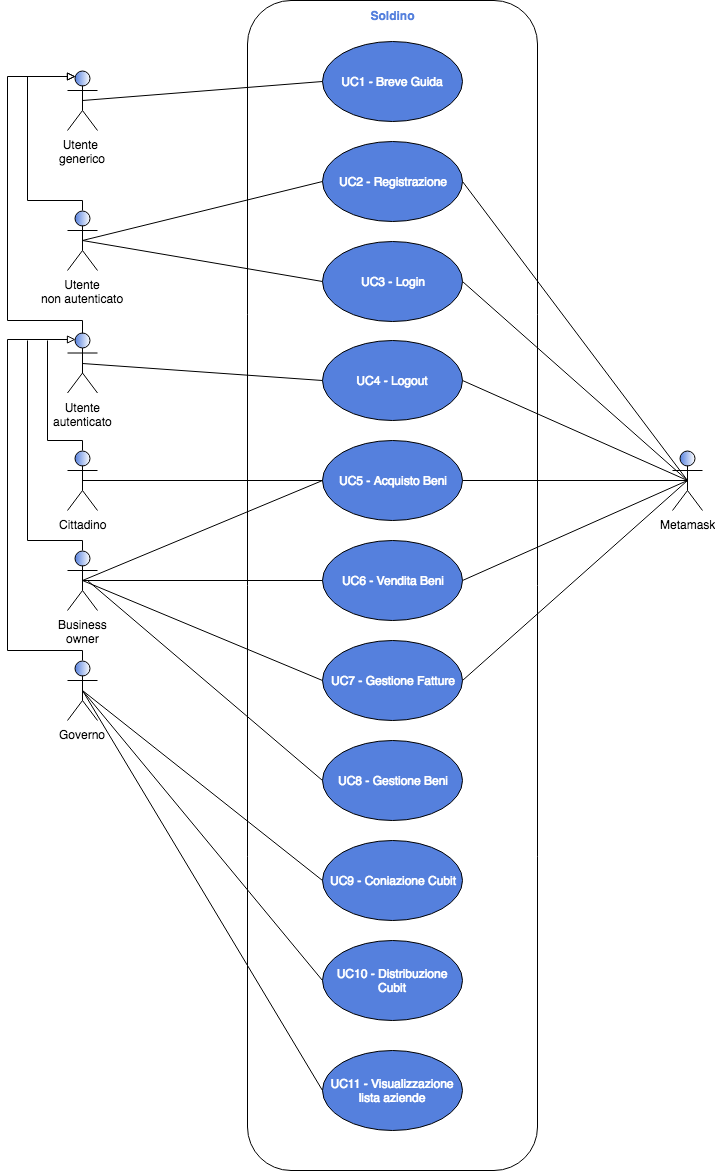
\includegraphics[width=9.38cm]{res/images/Elenco_casi_d_uso.png}
	\centering
	\caption{Elenco dei casi d'uso}
\end{figure}
\subsubsection{UC1 - Breve Guida}
\begin{itemize}
	\item \textbf{Attori Primari}
	\item \textbf{Descrizione}
	\item \textbf{Precondizione}
	\item \textbf{Postcondizione}
	\item \textbf{Scenario}
\end{itemize}
\subsubsection{UC2 - Registrazione}
\begin{itemize}
	\item \textbf{Attori Primari}
	\item \textbf{Descrizione}
	\item \textbf{Precondizione}
	\item \textbf{Postcondizione}
	\item \textbf{Scenario}
\end{itemize}
\subsubsection{UC3 - Login}
\begin{figure}[h]
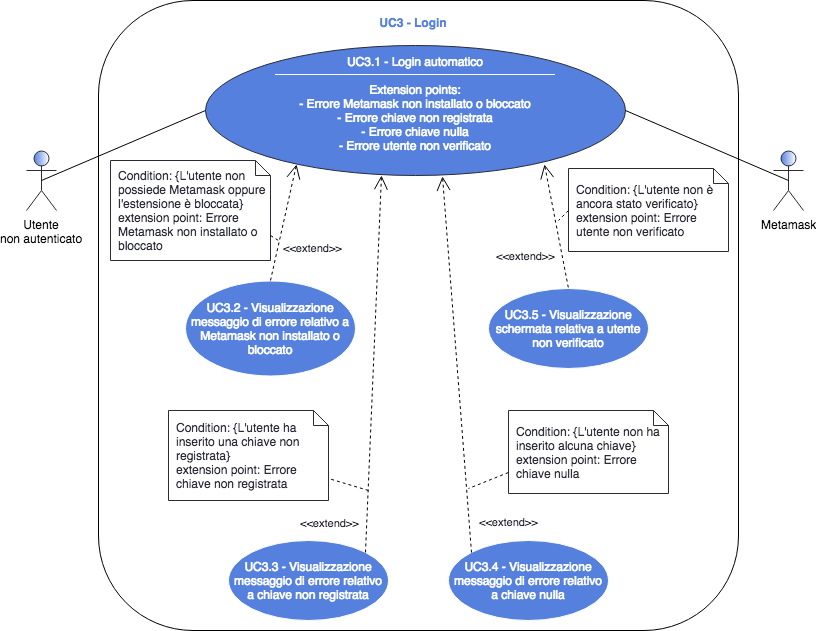
\includegraphics[width=14.5cm]{res/images/UC3Login.png}
\centering
\caption{UC3 - Login}

\end{figure}
\begin{itemize}
	\item \textbf{Attori Primari}
	Utente non autenticato
	\item \textbf{Attori Secondari}
	MetaMask\glo{}
	\item \textbf{Descrizione}
	L'utente prova a farsi identificare tramite l'interfaccia web per mezzo di MetaMask\glo{}.
	\item \textbf{Precondizione}
	L'utente non è identificato dalla piattaforma web.
	\item \textbf{Postcondizione}
	L'utente è identificato dalla piattaforma web. 
	\item \textbf{Scenario}
	L'utente non è identificato dal sito ed esegue il login.
\end{itemize}
\subsubsection{UC4 - Logout}
\begin{figure}[h]
	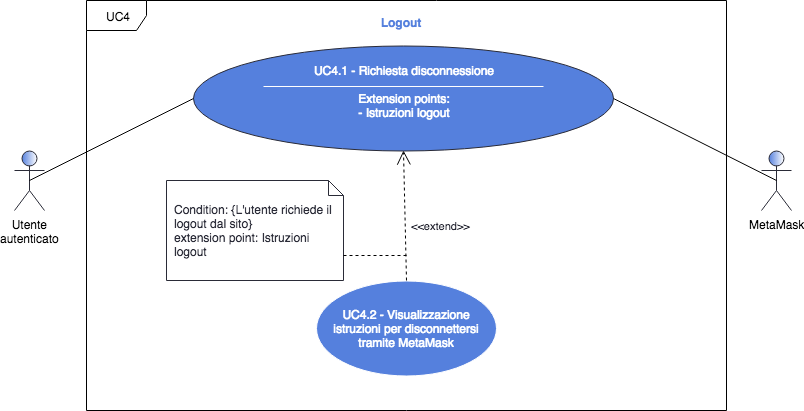
\includegraphics[width=14.5cm]{res/images/UC4Logout.png}
	\centering
	\caption{UC4 - Logout}
	
\end{figure}
\begin{itemize}
	\item \textbf{Attori Primari}
	Utente autenticato
	\item \textbf{Attori Secondari}
	MetaMask\glo{}
	\item \textbf{Descrizione}
	L'utente richiede il logout dalla piattaforma web ed effettua ciò tramite MetaMask\glo{}.
	\item \textbf{Precondizione}
	L'utente è identificato dalla piattaforma web e richiede di essere disconnesso dal sito.
	\item \textbf{Postcondizione}
	Vengono fornite le istruzioni necessarie per affrontare il Logout tramite MetaMask\glo{}. 
	\item \textbf{Scenario}
	L'utente è identificato dal sito ed esegue il logout.
\end{itemize}
\subsubsection{UC5 - Acquisto Beni}
\begin{itemize}
	\item \textbf{Attori Primari}
	\item \textbf{Descrizione}
	\item \textbf{Precondizione}
	\item \textbf{Postcondizione}
	\item \textbf{Scenario}
\end{itemize}
\subsubsection{UC6 - Vendita Beni}
\begin{itemize}
	\item \textbf{Attori Primari}
	\item \textbf{Descrizione}
	\item \textbf{Precondizione}
	\item \textbf{Postcondizione}
	\item \textbf{Scenario}
\end{itemize}
\subsubsection{UC7 - Gestione Fatture}
\begin{itemize}
	\item \textbf{Attori Primari}
	\item \textbf{Descrizione}
	\item \textbf{Precondizione}
	\item \textbf{Postcondizione}
	\item \textbf{Scenario}
\end{itemize}
\subsubsection{UC8 - Gestione Beni}
\begin{itemize}
	\item \textbf{Attori Primari}
	\item \textbf{Descrizione}
	\item \textbf{Precondizione}
	\item \textbf{Postcondizione}
	\item \textbf{Scenario}
\end{itemize}
\subsubsection{UC9 -  Coniazione Cubit}
\begin{itemize}
	\item \textbf{Attori Primari}
	\item \textbf{Descrizione}
	\item \textbf{Precondizione}
	\item \textbf{Postcondizione}
	\item \textbf{Scenario}
\end{itemize}
\subsubsection{UC10 - Distribuzione Cubit}
\begin{itemize}
	\item \textbf{Attori Primari}
	\item \textbf{Descrizione}
	\item \textbf{Precondizione}
	\item \textbf{Postcondizione}
	\item \textbf{Scenario}
\end{itemize}
\subsubsection{UC11 - Visualizzazione Lista Aziende}
\begin{itemize}
	\item \textbf{Attori Primari}
	\item \textbf{Descrizione}
	\item \textbf{Precondizione}
	\item \textbf{Postcondizione}
	\item \textbf{Scenario}
\end{itemize}

